\documentclass{standalone}
\usepackage{tikz}
\usetikzlibrary{patterns, positioning}
\usepackage[sfdefault]{ClearSans} %% option 'sfdefault' activates Clear Sans as the default text font
\usepackage[T1]{fontenc}

\begin{document}
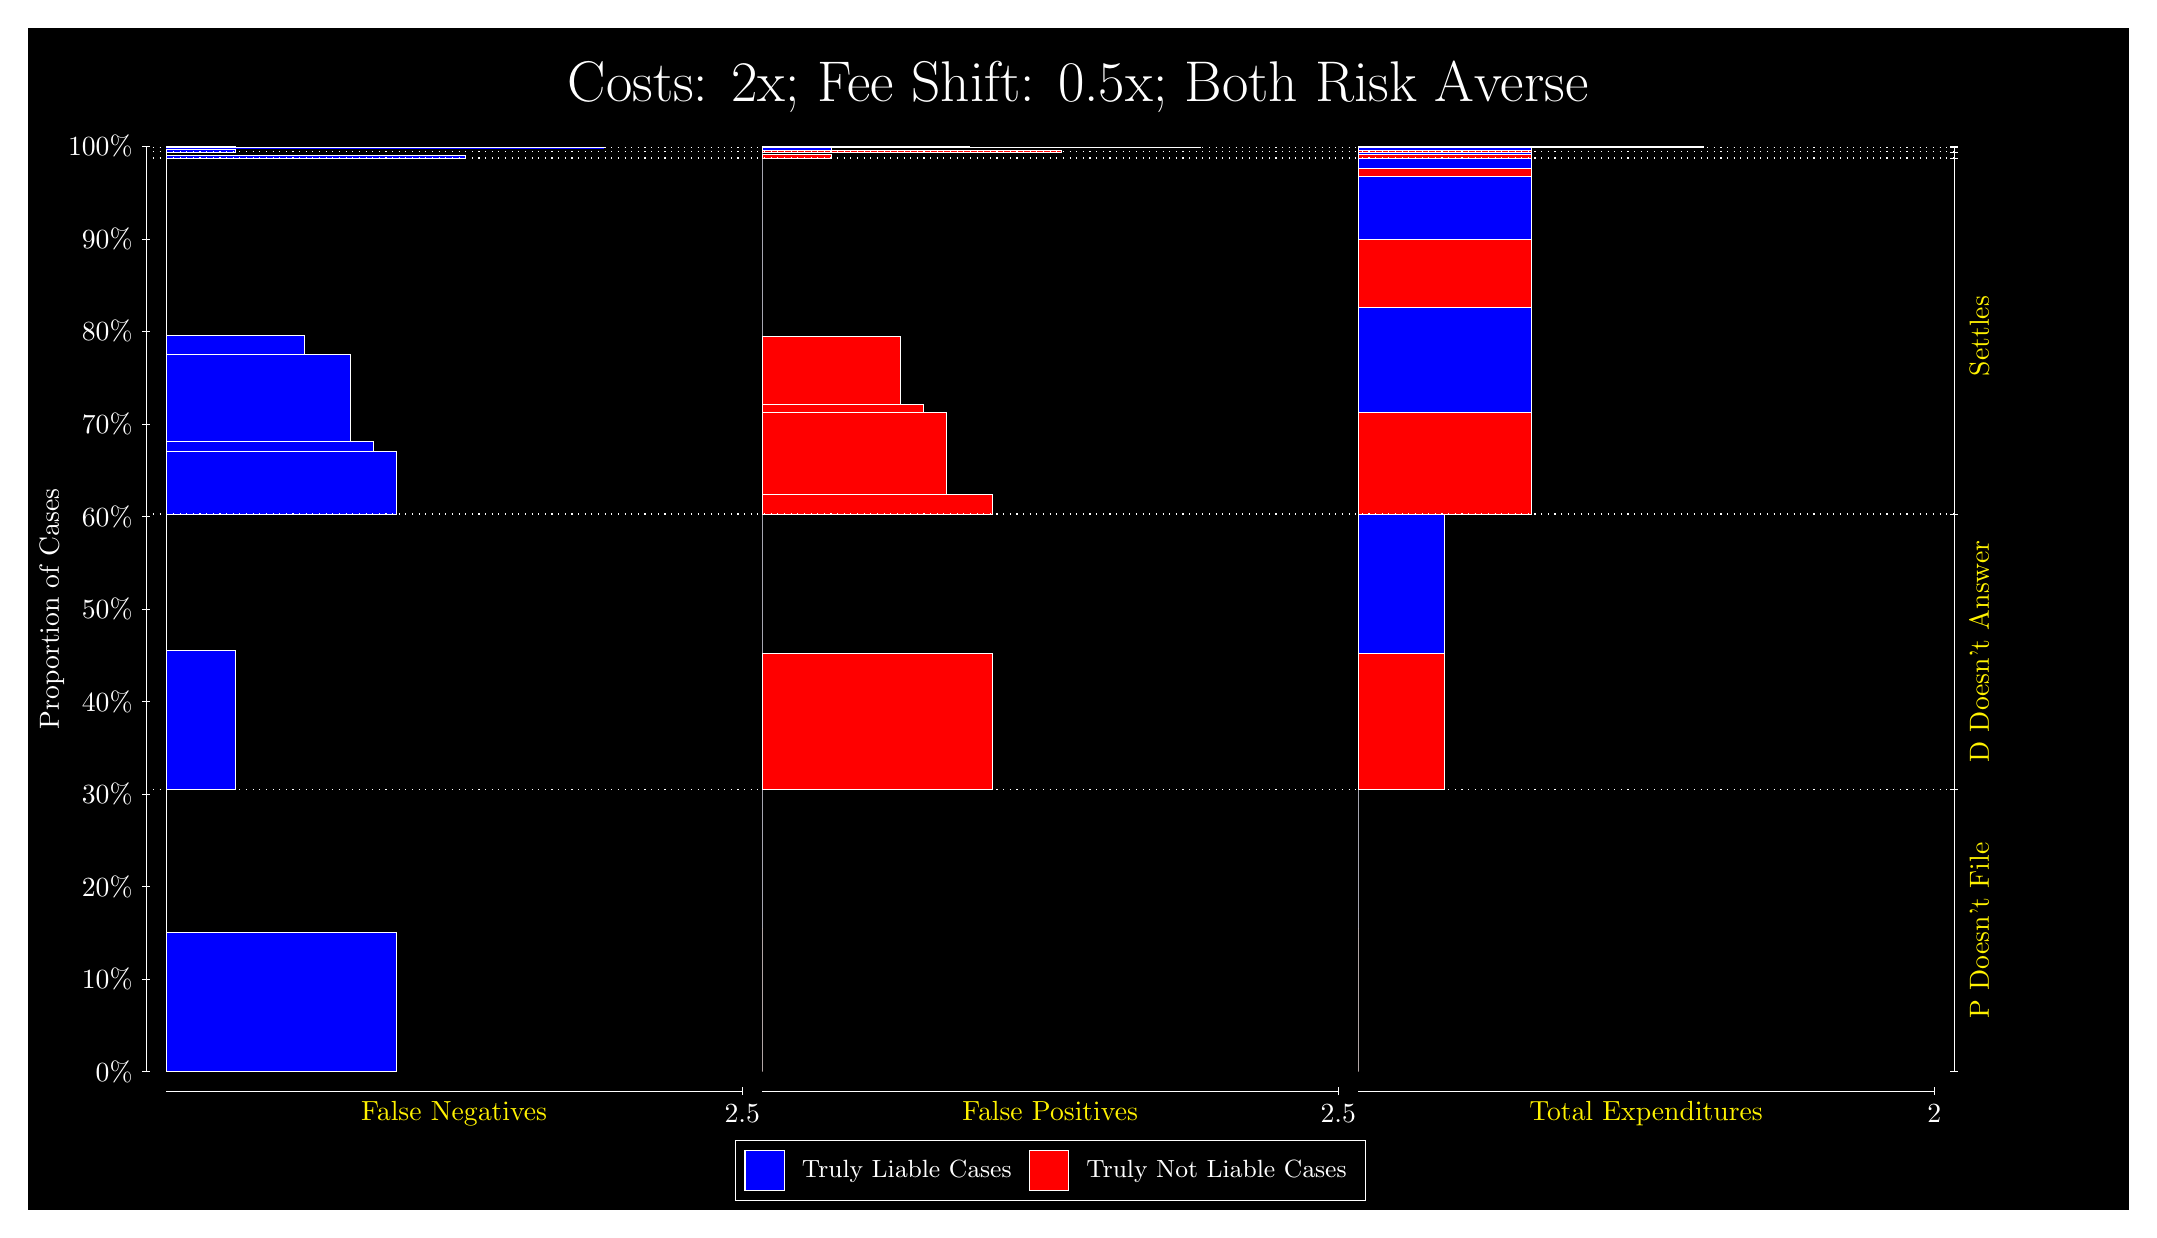
\begin{tikzpicture}
\draw[fill=black] (0,0) rectangle (26.667,15);
\draw[text=white] (0,13.5) rectangle (26.667,15) node[midway] {\huge Costs: 2x; Fee Shift: 0.5x; Both Risk Averse};
\draw[white, very thin] (1.5,1.75) -- (1.5,13.5);
\node[rotate=90, text=white, anchor=center] at (0.3, 7.625) {Proportion of Cases};
\draw[white, very thin] (1.45,1.75) -- (1.55,1.75);
\node[text=white, anchor=east] at (1.45, 1.75) {0\%};
\draw[white, very thin] (1.45,2.925) -- (1.55,2.925);
\node[text=white, anchor=east] at (1.45, 2.925) {10\%};
\draw[white, very thin] (1.45,4.1) -- (1.55,4.1);
\node[text=white, anchor=east] at (1.45, 4.1) {20\%};
\draw[white, very thin] (1.45,5.275) -- (1.55,5.275);
\node[text=white, anchor=east] at (1.45, 5.275) {30\%};
\draw[white, very thin] (1.45,6.45) -- (1.55,6.45);
\node[text=white, anchor=east] at (1.45, 6.45) {40\%};
\draw[white, very thin] (1.45,7.625) -- (1.55,7.625);
\node[text=white, anchor=east] at (1.45, 7.625) {50\%};
\draw[white, very thin] (1.45,8.8) -- (1.55,8.8);
\node[text=white, anchor=east] at (1.45, 8.8) {60\%};
\draw[white, very thin] (1.45,9.975) -- (1.55,9.975);
\node[text=white, anchor=east] at (1.45, 9.975) {70\%};
\draw[white, very thin] (1.45,11.15) -- (1.55,11.15);
\node[text=white, anchor=east] at (1.45, 11.15) {80\%};
\draw[white, very thin] (1.45,12.325) -- (1.55,12.325);
\node[text=white, anchor=east] at (1.45, 12.325) {90\%};
\draw[white, very thin] (1.45,13.5) -- (1.55,13.5);
\node[text=white, anchor=east] at (1.45, 13.5) {100\%};

\draw[white, very thin] (24.457,1.75) -- (24.457,13.5);
\draw[white, very thin] (24.407,1.75) -- (24.507,1.75);
\node[anchor=west] at (24.407, 1.75) {};
\draw[white, very thin] (24.407,5.3374) -- (24.507,5.3374);
\node[anchor=west] at (24.407, 5.3374) {};
\draw[white, very thin] (24.407,8.8302) -- (24.507,8.8302);
\node[anchor=west] at (24.407, 8.8302) {};
\draw[white, very thin] (24.407,13.352) -- (24.507,13.352);
\node[anchor=west] at (24.407, 13.352) {};
\draw[white, very thin] (24.407,13.43) -- (24.507,13.43);
\node[anchor=west] at (24.407, 13.43) {};
\draw[white, very thin] (24.407,13.482) -- (24.507,13.482);
\node[anchor=west] at (24.407, 13.482) {};
\draw[white, very thin] (24.407,13.49) -- (24.507,13.49);
\node[anchor=west] at (24.407, 13.49) {};
\draw[white, very thin] (24.407,13.5) -- (24.507,13.5);
\node[anchor=west] at (24.407, 13.5) {};

\draw[white, very thin, fill=blue] (1.75,1.75) rectangle (4.6775,3.5153);
\draw[white, very thin, fill=red] (1.75,3.5153) rectangle (1.75,5.3374);
\draw[white, very thin, fill=blue] (1.75,5.3374) rectangle (2.6283,7.1019);
\draw[white, very thin, fill=red] (1.75,7.1019) rectangle (1.75,8.8302);
\draw[white, very thin, fill=blue] (1.75,8.8302) rectangle (4.6775,9.6227);
\draw[white, very thin, fill=blue] (1.75,9.6227) rectangle (4.3848,9.7597);
\draw[white, very thin, fill=blue] (1.75,9.7597) rectangle (4.092,10.853);
\draw[white, very thin, fill=blue] (1.75,10.853) rectangle (3.5065,11.098);
\draw[white, very thin, fill=red] (1.75,11.098) rectangle (1.75,13.352);
\draw[white, very thin, fill=blue] (1.75,13.352) rectangle (5.5558,13.382);
\draw[white, very thin, fill=red] (1.75,13.382) rectangle (1.75,13.43);
\draw[white, very thin, fill=blue] (1.75,13.43) rectangle (2.6283,13.467);
\draw[white, very thin, fill=red] (1.75,13.467) rectangle (1.75,13.482);
\draw[white, very thin, fill=blue] (1.75,13.482) rectangle (7.3123,13.485);
\draw[white, very thin, fill=red] (1.75,13.485) rectangle (1.75,13.49);
\draw[white, very thin, fill=blue] (1.75,13.49) rectangle (2.6283,13.497);
\draw[white, very thin, fill=red] (1.75,13.497) rectangle (1.75,13.5);
\draw[white, very thin, fill=red] (9.3189,1.75) rectangle (9.3189,3.5721);
\draw[white, very thin, fill=blue] (9.3189,3.5721) rectangle (9.3189,5.3374);
\draw[white, very thin, fill=red] (9.3189,5.3374) rectangle (12.246,7.0657);
\draw[white, very thin, fill=blue] (9.3189,7.0657) rectangle (9.3189,8.8302);
\draw[white, very thin, fill=red] (9.3189,8.8302) rectangle (12.246,9.075);
\draw[white, very thin, fill=red] (9.3189,9.075) rectangle (11.661,10.123);
\draw[white, very thin, fill=red] (9.3189,10.123) rectangle (11.368,10.224);
\draw[white, very thin, fill=red] (9.3189,10.224) rectangle (11.075,11.084);
\draw[white, very thin, fill=blue] (9.3189,11.084) rectangle (9.3189,13.352);
\draw[white, very thin, fill=red] (9.3189,13.352) rectangle (10.197,13.4);
\draw[white, very thin, fill=blue] (9.3189,13.4) rectangle (9.3189,13.43);
\draw[white, very thin, fill=red] (9.3189,13.43) rectangle (13.125,13.444);
\draw[white, very thin, fill=blue] (9.3189,13.444) rectangle (10.197,13.482);
\draw[white, very thin, fill=red] (9.3189,13.482) rectangle (10.197,13.487);
\draw[white, very thin, fill=blue] (9.3189,13.487) rectangle (9.3189,13.49);
\draw[white, very thin, fill=red] (9.3189,13.49) rectangle (14.881,13.494);
\draw[white, very thin, fill=blue] (9.3189,13.494) rectangle (11.954,13.5);
\draw[white, very thin, fill=red] (16.888,1.75) rectangle (16.888,3.5721);
\draw[white, very thin, fill=blue] (16.888,3.5721) rectangle (16.888,5.3374);
\draw[white, very thin, fill=red] (16.888,5.3374) rectangle (17.986,7.0657);
\draw[white, very thin, fill=blue] (16.888,7.0657) rectangle (17.986,8.8302);
\draw[white, very thin, fill=red] (16.888,8.8302) rectangle (19.083,10.123);
\draw[white, very thin, fill=blue] (16.888,10.123) rectangle (19.083,11.462);
\draw[white, very thin, fill=red] (16.888,11.462) rectangle (19.083,12.322);
\draw[white, very thin, fill=blue] (16.888,12.322) rectangle (19.083,13.114);
\draw[white, very thin, fill=red] (16.888,13.114) rectangle (19.083,13.215);
\draw[white, very thin, fill=blue] (16.888,13.215) rectangle (19.083,13.352);
\draw[white, very thin, fill=red] (16.888,13.352) rectangle (19.083,13.4);
\draw[white, very thin, fill=blue] (16.888,13.4) rectangle (19.083,13.43);
\draw[white, very thin, fill=red] (16.888,13.43) rectangle (19.083,13.444);
\draw[white, very thin, fill=blue] (16.888,13.444) rectangle (19.083,13.482);
\draw[white, very thin, fill=red] (16.888,13.482) rectangle (21.279,13.487);
\draw[white, very thin, fill=blue] (16.888,13.487) rectangle (21.279,13.49);
\draw[white, very thin, fill=red] (16.888,13.49) rectangle (21.279,13.494);
\draw[white, very thin, fill=blue] (16.888,13.494) rectangle (21.279,13.5);
\draw[white, dotted] (1.5,5.3374) -- (24.457,5.3374);
\draw[white, dotted] (1.5,8.8302) -- (24.457,8.8302);
\draw[white, dotted] (1.5,13.352) -- (24.457,13.352);
\draw[white, dotted] (1.5,13.43) -- (24.457,13.43);
\draw[white, dotted] (1.5,13.482) -- (24.457,13.482);
\draw[white, dotted] (1.5,13.49) -- (24.457,13.49);
\draw[white, very thin] (1.75,1.5) -- (9.0689,1.5);
\node[text=yellow, anchor=north] at (5.4094, 1.5) {False Negatives};
\draw[white, very thin] (9.0689,1.45) -- (9.0689,1.55);
\node[text=white, anchor=north] at (9.0689, 1.45) {2.5};

\draw[white, very thin] (9.3189,1.5) -- (16.638,1.5);
\node[text=yellow, anchor=north] at (12.978, 1.5) {False Positives};
\draw[white, very thin] (16.638,1.45) -- (16.638,1.55);
\node[text=white, anchor=north] at (16.638, 1.45) {2.5};

\draw[white, very thin] (16.888,1.5) -- (24.207,1.5);
\node[text=yellow, anchor=north] at (20.547, 1.5) {Total Expenditures};
\draw[white, very thin] (24.207,1.45) -- (24.207,1.55);
\node[text=white, anchor=north] at (24.207, 1.45) {2};

\node[text=yellow, centered, rotate=90] at (24.777, 3.5437) {P Doesn't File};
\node[text=yellow, centered, rotate=90] at (24.777, 7.0838) {D Doesn't Answer};
\node[text=yellow, centered, rotate=90] at (24.777, 11.091) {Settles};





\draw (12.978300999999998,1.5) node[draw=none] (baseCoordinate) {};
\begin{scope}[align=center]
        \matrix[scale=0.5, draw=white, below=0.5cm of baseCoordinate, nodes={draw}, column sep=0.1cm]{
            \node[rectangle, draw, minimum width=0.5cm, minimum height=0.5cm, fill=blue] {}; &
            \node[draw=none, font=\small, text=white] (B) {Truly Liable Cases}; &
            \node[rectangle, draw, minimum width=0.5cm, minimum height=0.5cm, fill=red] {}; &
            \node[draw=none, font=\small, text=white] (B) {Truly Not Liable Cases}; \\
            };
\end{scope}

\end{tikzpicture}
\end{document}